\subsection{Calibrazione}
Un primo passo necessario per la successiva analisi dati vera e propria è la calibrazione dei sistema di acquisizione, effettuata tramite una conoscenza a priori dell'energia
associata ai fotoni emessi dalla sorgente. I fotoni utilizzati a tale scopo sono quelli relativi alla cascata gamma successiva al decadimento $\beta$ del nucleo di \isotope{Co}{60}, ovvero
i gamma con energia pari a 1173 keV e 1333 keV. Per ogni rivelatore è stato quindi acquisito uno spettro in cui fossero visibili i picchi associati a tali gamma che sono stati
successivamente fittati in maniera tale da potervici associare un centroide. A questo punto avendo due coppie di valori per rivelatore sarebbe in linea di principio possibile
ottenere una relazione lineare che permette di calibrare lo spettro, ma essendo i centroidi trovati di valore molto grande $\approx 10^4$ e relativamente molto vicini, ciò
porterebbe ad una grande incertezza sul parametro di ordine 0 del fit. Si è quindi acquisito un ulteriore spettro relativo ad una sorgente di \isotope{Am}{241} 
che presenta 
un picco a 59.5 keV, ottenendo in tal modo un terzo punto per la calibrazione. Di seguito i punti ottenuti per la calibrazione ed i parametri ricavati dal fit. I risultati sono
per il rivelatore 1:
$$ m = (0.1046 \pm 0.0002) \text{keV}\hspace{2cm} q = (0.6 \pm 2) \text{keV}$$
mentre per il riveltore 2 si ha:
$$ m = (0.1092 \pm 0.0009) \text{keV}\hspace{2cm} q = (0.3 \pm 8) \text{keV}$$
Per quanto riguarda le interpolazioni dei singoli fotopicchi si rimanda alle appendici.

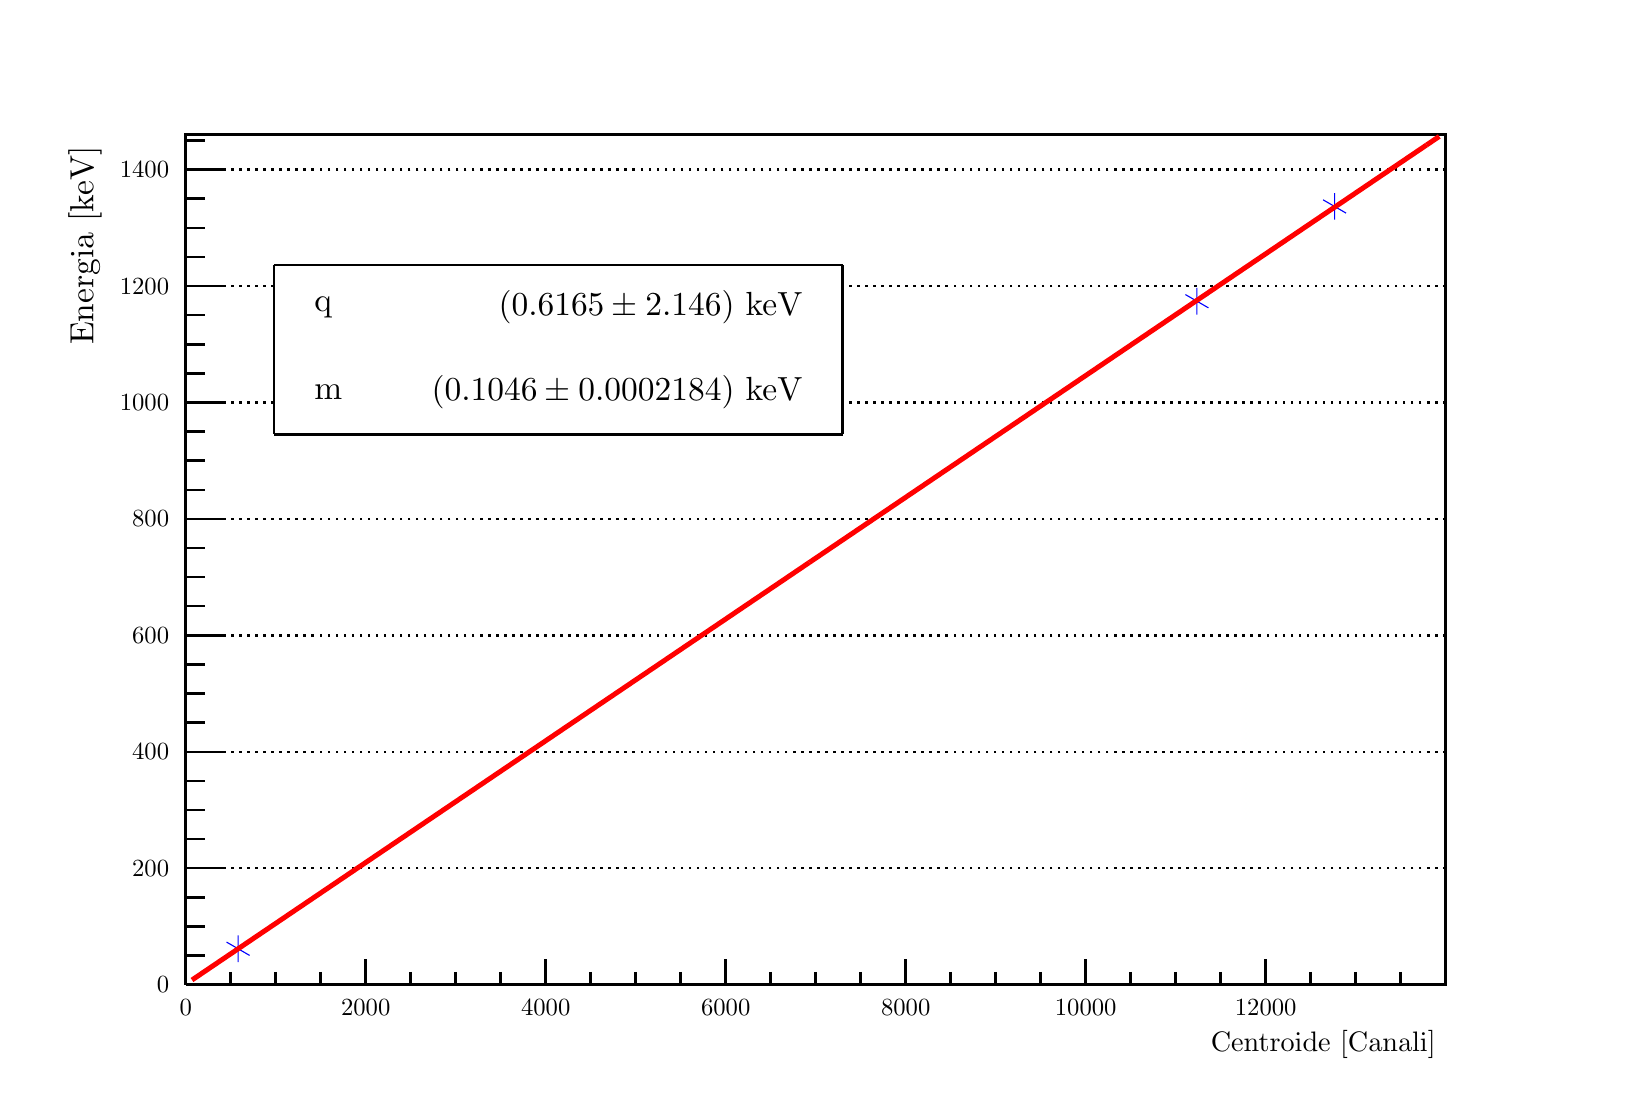
\begin{tikzpicture}
\pgfdeclareplotmark{cross} {
\pgfpathmoveto{\pgfpoint{-0.3\pgfplotmarksize}{\pgfplotmarksize}}
\pgfpathlineto{\pgfpoint{+0.3\pgfplotmarksize}{\pgfplotmarksize}}
\pgfpathlineto{\pgfpoint{+0.3\pgfplotmarksize}{0.3\pgfplotmarksize}}
\pgfpathlineto{\pgfpoint{+1\pgfplotmarksize}{0.3\pgfplotmarksize}}
\pgfpathlineto{\pgfpoint{+1\pgfplotmarksize}{-0.3\pgfplotmarksize}}
\pgfpathlineto{\pgfpoint{+0.3\pgfplotmarksize}{-0.3\pgfplotmarksize}}
\pgfpathlineto{\pgfpoint{+0.3\pgfplotmarksize}{-1.\pgfplotmarksize}}
\pgfpathlineto{\pgfpoint{-0.3\pgfplotmarksize}{-1.\pgfplotmarksize}}
\pgfpathlineto{\pgfpoint{-0.3\pgfplotmarksize}{-0.3\pgfplotmarksize}}
\pgfpathlineto{\pgfpoint{-1.\pgfplotmarksize}{-0.3\pgfplotmarksize}}
\pgfpathlineto{\pgfpoint{-1.\pgfplotmarksize}{0.3\pgfplotmarksize}}
\pgfpathlineto{\pgfpoint{-0.3\pgfplotmarksize}{0.3\pgfplotmarksize}}
\pgfpathclose
\pgfusepathqstroke
}
\pgfdeclareplotmark{cross*} {
\pgfpathmoveto{\pgfpoint{-0.3\pgfplotmarksize}{\pgfplotmarksize}}
\pgfpathlineto{\pgfpoint{+0.3\pgfplotmarksize}{\pgfplotmarksize}}
\pgfpathlineto{\pgfpoint{+0.3\pgfplotmarksize}{0.3\pgfplotmarksize}}
\pgfpathlineto{\pgfpoint{+1\pgfplotmarksize}{0.3\pgfplotmarksize}}
\pgfpathlineto{\pgfpoint{+1\pgfplotmarksize}{-0.3\pgfplotmarksize}}
\pgfpathlineto{\pgfpoint{+0.3\pgfplotmarksize}{-0.3\pgfplotmarksize}}
\pgfpathlineto{\pgfpoint{+0.3\pgfplotmarksize}{-1.\pgfplotmarksize}}
\pgfpathlineto{\pgfpoint{-0.3\pgfplotmarksize}{-1.\pgfplotmarksize}}
\pgfpathlineto{\pgfpoint{-0.3\pgfplotmarksize}{-0.3\pgfplotmarksize}}
\pgfpathlineto{\pgfpoint{-1.\pgfplotmarksize}{-0.3\pgfplotmarksize}}
\pgfpathlineto{\pgfpoint{-1.\pgfplotmarksize}{0.3\pgfplotmarksize}}
\pgfpathlineto{\pgfpoint{-0.3\pgfplotmarksize}{0.3\pgfplotmarksize}}
\pgfpathclose
\pgfusepathqfillstroke
}
\pgfdeclareplotmark{newstar} {
\pgfpathmoveto{\pgfqpoint{0pt}{\pgfplotmarksize}}
\pgfpathlineto{\pgfqpointpolar{44}{0.5\pgfplotmarksize}}
\pgfpathlineto{\pgfqpointpolar{18}{\pgfplotmarksize}}
\pgfpathlineto{\pgfqpointpolar{-20}{0.5\pgfplotmarksize}}
\pgfpathlineto{\pgfqpointpolar{-54}{\pgfplotmarksize}}
\pgfpathlineto{\pgfqpointpolar{-90}{0.5\pgfplotmarksize}}
\pgfpathlineto{\pgfqpointpolar{234}{\pgfplotmarksize}}
\pgfpathlineto{\pgfqpointpolar{198}{0.5\pgfplotmarksize}}
\pgfpathlineto{\pgfqpointpolar{162}{\pgfplotmarksize}}
\pgfpathlineto{\pgfqpointpolar{134}{0.5\pgfplotmarksize}}
\pgfpathclose
\pgfusepathqstroke
}
\pgfdeclareplotmark{newstar*} {
\pgfpathmoveto{\pgfqpoint{0pt}{\pgfplotmarksize}}
\pgfpathlineto{\pgfqpointpolar{44}{0.5\pgfplotmarksize}}
\pgfpathlineto{\pgfqpointpolar{18}{\pgfplotmarksize}}
\pgfpathlineto{\pgfqpointpolar{-20}{0.5\pgfplotmarksize}}
\pgfpathlineto{\pgfqpointpolar{-54}{\pgfplotmarksize}}
\pgfpathlineto{\pgfqpointpolar{-90}{0.5\pgfplotmarksize}}
\pgfpathlineto{\pgfqpointpolar{234}{\pgfplotmarksize}}
\pgfpathlineto{\pgfqpointpolar{198}{0.5\pgfplotmarksize}}
\pgfpathlineto{\pgfqpointpolar{162}{\pgfplotmarksize}}
\pgfpathlineto{\pgfqpointpolar{134}{0.5\pgfplotmarksize}}
\pgfpathclose
\pgfusepathqfillstroke
}
\definecolor{c}{rgb}{1,1,1};
\draw [color=c, fill=c] (0,0) rectangle (20,13.4957);
\draw [color=c, fill=c] (2,1.34957) rectangle (18,12.1461);
\definecolor{c}{rgb}{0,0,0};
\draw [c,line width=0.9] (2,1.34957) -- (2,12.1461) -- (18,12.1461) -- (18,1.34957) -- (2,1.34957);
\definecolor{c}{rgb}{1,1,1};
\draw [color=c, fill=c] (2,1.34957) rectangle (18,12.1461);
\definecolor{c}{rgb}{0,0,0};
\draw [c,line width=0.9] (2,1.34957) -- (2,12.1461) -- (18,12.1461) -- (18,1.34957) -- (2,1.34957);
\draw [c,line width=0.9] (2,1.34957) -- (18,1.34957);
\draw [c,line width=0.9] (2,1.34957) -- (2,12.1461);
\draw [c,dotted,line width=0.9] (18,1.34957) -- (2,1.34957);
\draw [c,dotted,line width=0.9] (18,2.8282) -- (2,2.8282);
\draw [c,dotted,line width=0.9] (18,4.30682) -- (2,4.30682);
\draw [c,dotted,line width=0.9] (18,5.78545) -- (2,5.78545);
\draw [c,dotted,line width=0.9] (18,7.26408) -- (2,7.26408);
\draw [c,dotted,line width=0.9] (18,8.7427) -- (2,8.7427);
\draw [c,dotted,line width=0.9] (18,10.2213) -- (2,10.2213);
\draw [c,dotted,line width=0.9] (18,11.7) -- (2,11.7);
\draw [c,dotted,line width=0.9] (18,11.7) -- (2,11.7);
\draw [c,line width=0.9] (2,1.34957) -- (18,1.34957);
\draw [anchor= east] (18,0.593811) node[scale=1.01821, color=c, rotate=0]{Centroide [Canali]};
\draw [c,line width=0.9] (2,1.67347) -- (2,1.34957);
\draw [c,line width=0.9] (2.57151,1.51152) -- (2.57151,1.34957);
\draw [c,line width=0.9] (3.14302,1.51152) -- (3.14302,1.34957);
\draw [c,line width=0.9] (3.71452,1.51152) -- (3.71452,1.34957);
\draw [c,line width=0.9] (4.28603,1.67347) -- (4.28603,1.34957);
\draw [c,line width=0.9] (4.85754,1.51152) -- (4.85754,1.34957);
\draw [c,line width=0.9] (5.42905,1.51152) -- (5.42905,1.34957);
\draw [c,line width=0.9] (6.00056,1.51152) -- (6.00056,1.34957);
\draw [c,line width=0.9] (6.57207,1.67347) -- (6.57207,1.34957);
\draw [c,line width=0.9] (7.14357,1.51152) -- (7.14357,1.34957);
\draw [c,line width=0.9] (7.71508,1.51152) -- (7.71508,1.34957);
\draw [c,line width=0.9] (8.28659,1.51152) -- (8.28659,1.34957);
\draw [c,line width=0.9] (8.8581,1.67347) -- (8.8581,1.34957);
\draw [c,line width=0.9] (9.42961,1.51152) -- (9.42961,1.34957);
\draw [c,line width=0.9] (10.0011,1.51152) -- (10.0011,1.34957);
\draw [c,line width=0.9] (10.5726,1.51152) -- (10.5726,1.34957);
\draw [c,line width=0.9] (11.1441,1.67347) -- (11.1441,1.34957);
\draw [c,line width=0.9] (11.7156,1.51152) -- (11.7156,1.34957);
\draw [c,line width=0.9] (12.2871,1.51152) -- (12.2871,1.34957);
\draw [c,line width=0.9] (12.8587,1.51152) -- (12.8587,1.34957);
\draw [c,line width=0.9] (13.4302,1.67347) -- (13.4302,1.34957);
\draw [c,line width=0.9] (14.0017,1.51152) -- (14.0017,1.34957);
\draw [c,line width=0.9] (14.5732,1.51152) -- (14.5732,1.34957);
\draw [c,line width=0.9] (15.1447,1.51152) -- (15.1447,1.34957);
\draw [c,line width=0.9] (15.7162,1.67347) -- (15.7162,1.34957);
\draw [c,line width=0.9] (15.7162,1.67347) -- (15.7162,1.34957);
\draw [c,line width=0.9] (16.2877,1.51152) -- (16.2877,1.34957);
\draw [c,line width=0.9] (16.8592,1.51152) -- (16.8592,1.34957);
\draw [c,line width=0.9] (17.4307,1.51152) -- (17.4307,1.34957);
\draw [anchor=base] (2,0.958195) node[scale=0.890934, color=c, rotate=0]{0};
\draw [anchor=base] (4.28603,0.958195) node[scale=0.890934, color=c, rotate=0]{2000};
\draw [anchor=base] (6.57207,0.958195) node[scale=0.890934, color=c, rotate=0]{4000};
\draw [anchor=base] (8.8581,0.958195) node[scale=0.890934, color=c, rotate=0]{6000};
\draw [anchor=base] (11.1441,0.958195) node[scale=0.890934, color=c, rotate=0]{8000};
\draw [anchor=base] (13.4302,0.958195) node[scale=0.890934, color=c, rotate=0]{10000};
\draw [anchor=base] (15.7162,0.958195) node[scale=0.890934, color=c, rotate=0]{12000};
\draw [c,line width=0.9] (2,1.34957) -- (2,12.1461);
\draw [anchor= east] (0.72,12.1461) node[scale=1.20912, color=c, rotate=90]{Energia [keV]};
\draw [c,line width=0.9] (2.48,1.34957) -- (2,1.34957);
\draw [c,line width=0.9] (2.24,1.71923) -- (2,1.71923);
\draw [c,line width=0.9] (2.24,2.08888) -- (2,2.08888);
\draw [c,line width=0.9] (2.24,2.45854) -- (2,2.45854);
\draw [c,line width=0.9] (2.48,2.8282) -- (2,2.8282);
\draw [c,line width=0.9] (2.24,3.19785) -- (2,3.19785);
\draw [c,line width=0.9] (2.24,3.56751) -- (2,3.56751);
\draw [c,line width=0.9] (2.24,3.93717) -- (2,3.93717);
\draw [c,line width=0.9] (2.48,4.30682) -- (2,4.30682);
\draw [c,line width=0.9] (2.24,4.67648) -- (2,4.67648);
\draw [c,line width=0.9] (2.24,5.04614) -- (2,5.04614);
\draw [c,line width=0.9] (2.24,5.41579) -- (2,5.41579);
\draw [c,line width=0.9] (2.48,5.78545) -- (2,5.78545);
\draw [c,line width=0.9] (2.24,6.15511) -- (2,6.15511);
\draw [c,line width=0.9] (2.24,6.52476) -- (2,6.52476);
\draw [c,line width=0.9] (2.24,6.89442) -- (2,6.89442);
\draw [c,line width=0.9] (2.48,7.26408) -- (2,7.26408);
\draw [c,line width=0.9] (2.24,7.63373) -- (2,7.63373);
\draw [c,line width=0.9] (2.24,8.00339) -- (2,8.00339);
\draw [c,line width=0.9] (2.24,8.37305) -- (2,8.37305);
\draw [c,line width=0.9] (2.48,8.7427) -- (2,8.7427);
\draw [c,line width=0.9] (2.24,9.11236) -- (2,9.11236);
\draw [c,line width=0.9] (2.24,9.48202) -- (2,9.48202);
\draw [c,line width=0.9] (2.24,9.85167) -- (2,9.85167);
\draw [c,line width=0.9] (2.48,10.2213) -- (2,10.2213);
\draw [c,line width=0.9] (2.24,10.591) -- (2,10.591);
\draw [c,line width=0.9] (2.24,10.9606) -- (2,10.9606);
\draw [c,line width=0.9] (2.24,11.3303) -- (2,11.3303);
\draw [c,line width=0.9] (2.48,11.7) -- (2,11.7);
\draw [c,line width=0.9] (2.48,11.7) -- (2,11.7);
\draw [c,line width=0.9] (2.24,12.0696) -- (2,12.0696);
\draw [anchor= east] (1.9,1.34957) node[scale=0.890934, color=c, rotate=0]{0};
\draw [anchor= east] (1.9,2.8282) node[scale=0.890934, color=c, rotate=0]{200};
\draw [anchor= east] (1.9,4.30682) node[scale=0.890934, color=c, rotate=0]{400};
\draw [anchor= east] (1.9,5.78545) node[scale=0.890934, color=c, rotate=0]{600};
\draw [anchor= east] (1.9,7.26408) node[scale=0.890934, color=c, rotate=0]{800};
\draw [anchor= east] (1.9,8.7427) node[scale=0.890934, color=c, rotate=0]{1000};
\draw [anchor= east] (1.9,10.2213) node[scale=0.890934, color=c, rotate=0]{1200};
\draw [anchor= east] (1.9,11.7) node[scale=0.890934, color=c, rotate=0]{1400};
\definecolor{c}{rgb}{1,1,1};
\draw [color=c, fill=c] (3.12321,8.33811) rectangle (10.3438,10.4871);
\definecolor{c}{rgb}{0,0,0};
\draw [c,line width=0.9] (3.12321,8.33811) -- (10.3438,8.33811);
\draw [c,line width=0.9] (10.3438,8.33811) -- (10.3438,10.4871);
\draw [c,line width=0.9] (10.3438,10.4871) -- (3.12321,10.4871);
\draw [c,line width=0.9] (3.12321,10.4871) -- (3.12321,8.33811);
\draw [anchor= west] (3.48424,9.94986) node[scale=1.20912, color=c, rotate=0]{q       };
\draw [anchor= east] (9.98281,9.94986) node[scale=1.20912, color=c, rotate=0]{$ (0.6165 \pm 2.146)$ keV};
\draw [anchor= west] (3.48424,8.87536) node[scale=1.20912, color=c, rotate=0]{m       };
\draw [anchor= east] (9.98281,8.87536) node[scale=1.20912, color=c, rotate=0]{$ (0.1046 \pm 0.0002184)$ keV};
\definecolor{c}{rgb}{0,0,1};
\foreach \P in {(2.66476,1.80516),(14.8424,10.0287),(16.5903,11.2321)}{\draw[mark options={color=c,fill=c},mark size=4.804805pt,mark=asterisk] plot coordinates {\P};}
\definecolor{c}{rgb}{1,0,0};
\draw [c,line width=1.8] (2.08,1.40824) -- (2.24,1.51645) -- (2.4,1.62467) -- (2.56,1.73288) -- (2.72,1.8411) -- (2.88,1.94931) -- (3.04,2.05753) -- (3.2,2.16574) -- (3.36,2.27396) -- (3.52,2.38217) -- (3.68,2.49039) -- (3.84,2.5986) -- (4,2.70682)
 -- (4.16,2.81503) -- (4.32,2.92325) -- (4.48,3.03146) -- (4.64,3.13968) -- (4.8,3.24789) -- (4.96,3.35611) -- (5.12,3.46432) -- (5.28,3.57254) -- (5.44,3.68075) -- (5.6,3.78897) -- (5.76,3.89718) -- (5.92,4.0054) -- (6.08,4.11361) -- (6.24,4.22183)
 -- (6.4,4.33004) -- (6.56,4.43826) -- (6.72,4.54647) -- (6.88,4.65469) -- (7.04,4.7629) -- (7.2,4.87112) -- (7.36,4.97933) -- (7.52,5.08755) -- (7.68,5.19576) -- (7.84,5.30398) -- (8,5.41219) -- (8.16,5.52041) -- (8.32,5.62862) -- (8.48,5.73684) --
 (8.64,5.84505) -- (8.8,5.95327) -- (8.96,6.06148) -- (9.12,6.1697) -- (9.28,6.27791) -- (9.44,6.38613) -- (9.6,6.49434) -- (9.76,6.60256) -- (9.92,6.71077);
\draw [c,line width=1.8] (9.92,6.71077) -- (10.08,6.81899) -- (10.24,6.9272) -- (10.4,7.03542) -- (10.56,7.14363) -- (10.72,7.25185) -- (10.88,7.36006) -- (11.04,7.46828) -- (11.2,7.57649) -- (11.36,7.68471) -- (11.52,7.79292) -- (11.68,7.90114) --
 (11.84,8.00935) -- (12,8.11757) -- (12.16,8.22578) -- (12.32,8.334) -- (12.48,8.44221) -- (12.64,8.55043) -- (12.8,8.65864) -- (12.96,8.76686) -- (13.12,8.87507) -- (13.28,8.98329) -- (13.44,9.0915) -- (13.6,9.19972) -- (13.76,9.30793) --
 (13.92,9.41615) -- (14.08,9.52436) -- (14.24,9.63258) -- (14.4,9.74079) -- (14.56,9.84901) -- (14.72,9.95722) -- (14.88,10.0654) -- (15.04,10.1737) -- (15.2,10.2819) -- (15.36,10.3901) -- (15.52,10.4983) -- (15.68,10.6065) -- (15.84,10.7147) --
 (16,10.8229) -- (16.16,10.9312) -- (16.32,11.0394) -- (16.48,11.1476) -- (16.64,11.2558) -- (16.8,11.364) -- (16.96,11.4722) -- (17.12,11.5804) -- (17.28,11.6887) -- (17.44,11.7969) -- (17.6,11.9051) -- (17.76,12.0133);
\draw [c,line width=1.8] (17.76,12.0133) -- (17.92,12.1215);
\definecolor{c}{rgb}{1,1,1};
\draw [color=c, fill=c] (3.12321,8.33811) rectangle (10.3438,10.4871);
\definecolor{c}{rgb}{0,0,0};
\draw [c,line width=0.9] (3.12321,8.33811) -- (10.3438,8.33811);
\draw [c,line width=0.9] (10.3438,8.33811) -- (10.3438,10.4871);
\draw [c,line width=0.9] (10.3438,10.4871) -- (3.12321,10.4871);
\draw [c,line width=0.9] (3.12321,10.4871) -- (3.12321,8.33811);
\draw [anchor= west] (3.48424,9.94986) node[scale=1.20912, color=c, rotate=0]{q       };
\draw [anchor= east] (9.98281,9.94986) node[scale=1.20912, color=c, rotate=0]{$ (0.6165 \pm 2.146)$ keV};
\draw [anchor= west] (3.48424,8.87536) node[scale=1.20912, color=c, rotate=0]{m       };
\draw [anchor= east] (9.98281,8.87536) node[scale=1.20912, color=c, rotate=0]{$ (0.1046 \pm 0.0002184)$ keV};
\draw (9.51289,12.8653) node[scale=1.40004, color=c, rotate=0]{ };
\end{tikzpicture}

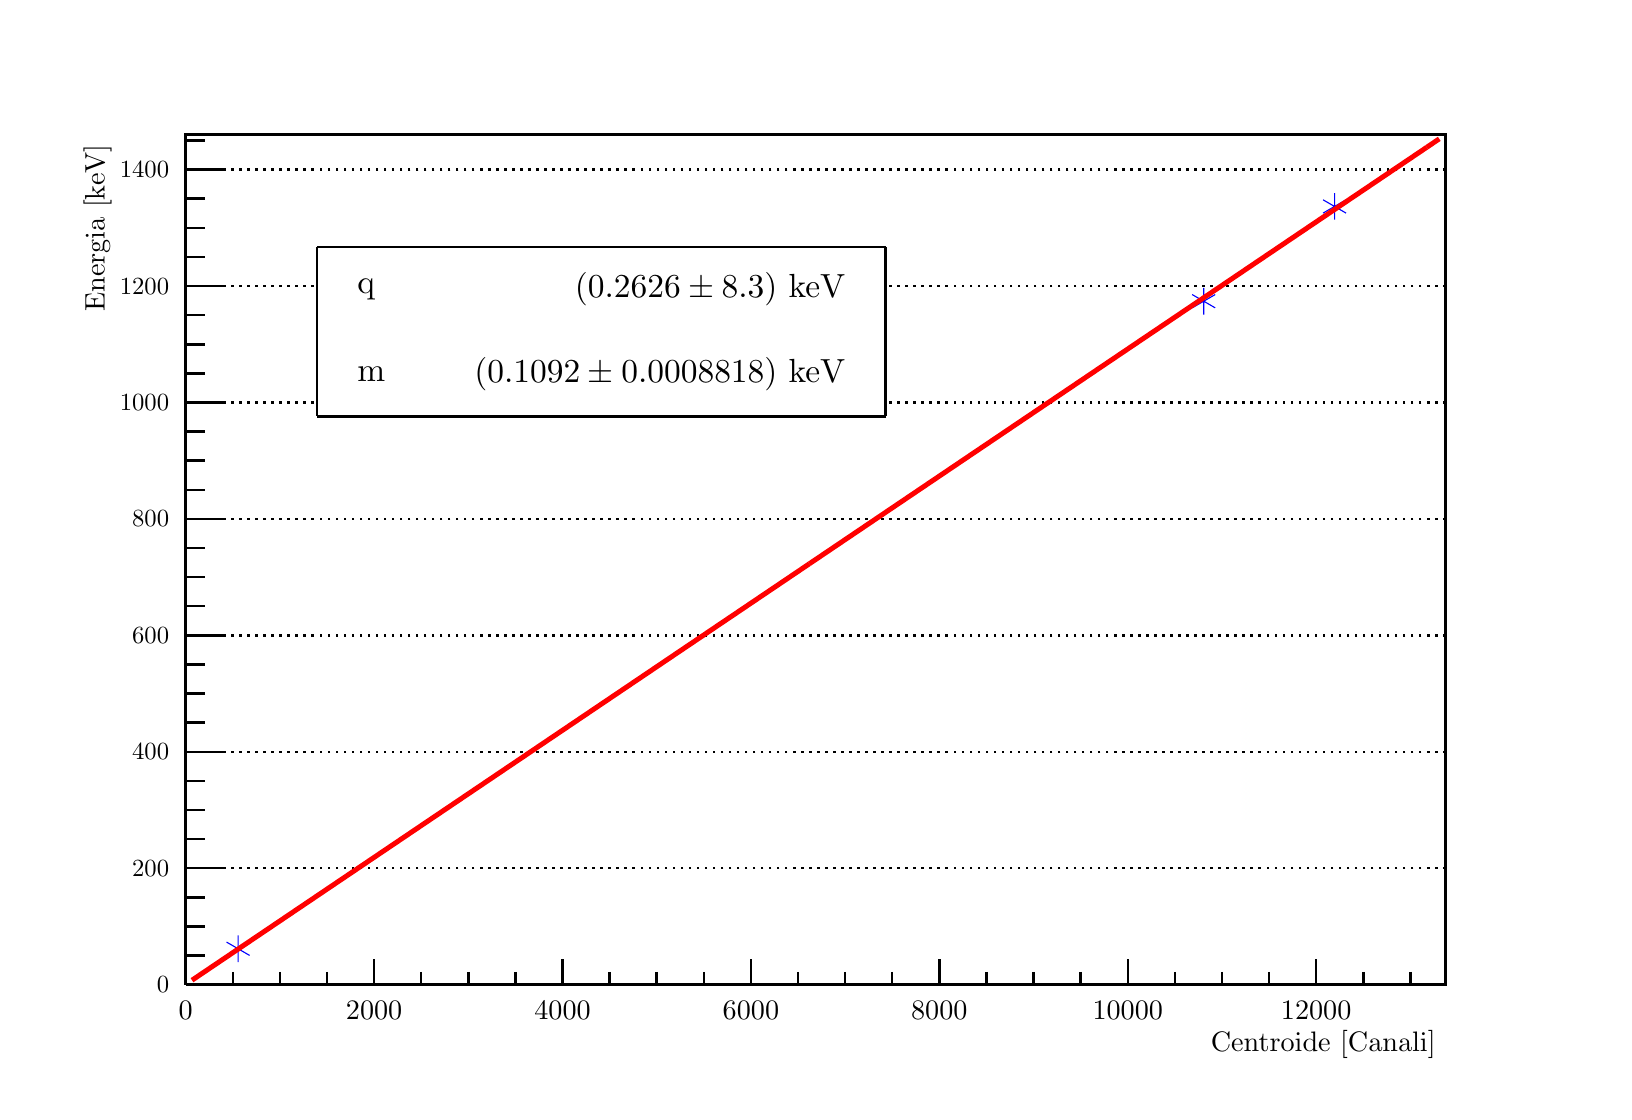
\begin{tikzpicture}
\pgfdeclareplotmark{cross} {
\pgfpathmoveto{\pgfpoint{-0.3\pgfplotmarksize}{\pgfplotmarksize}}
\pgfpathlineto{\pgfpoint{+0.3\pgfplotmarksize}{\pgfplotmarksize}}
\pgfpathlineto{\pgfpoint{+0.3\pgfplotmarksize}{0.3\pgfplotmarksize}}
\pgfpathlineto{\pgfpoint{+1\pgfplotmarksize}{0.3\pgfplotmarksize}}
\pgfpathlineto{\pgfpoint{+1\pgfplotmarksize}{-0.3\pgfplotmarksize}}
\pgfpathlineto{\pgfpoint{+0.3\pgfplotmarksize}{-0.3\pgfplotmarksize}}
\pgfpathlineto{\pgfpoint{+0.3\pgfplotmarksize}{-1.\pgfplotmarksize}}
\pgfpathlineto{\pgfpoint{-0.3\pgfplotmarksize}{-1.\pgfplotmarksize}}
\pgfpathlineto{\pgfpoint{-0.3\pgfplotmarksize}{-0.3\pgfplotmarksize}}
\pgfpathlineto{\pgfpoint{-1.\pgfplotmarksize}{-0.3\pgfplotmarksize}}
\pgfpathlineto{\pgfpoint{-1.\pgfplotmarksize}{0.3\pgfplotmarksize}}
\pgfpathlineto{\pgfpoint{-0.3\pgfplotmarksize}{0.3\pgfplotmarksize}}
\pgfpathclose
\pgfusepathqstroke
}
\pgfdeclareplotmark{cross*} {
\pgfpathmoveto{\pgfpoint{-0.3\pgfplotmarksize}{\pgfplotmarksize}}
\pgfpathlineto{\pgfpoint{+0.3\pgfplotmarksize}{\pgfplotmarksize}}
\pgfpathlineto{\pgfpoint{+0.3\pgfplotmarksize}{0.3\pgfplotmarksize}}
\pgfpathlineto{\pgfpoint{+1\pgfplotmarksize}{0.3\pgfplotmarksize}}
\pgfpathlineto{\pgfpoint{+1\pgfplotmarksize}{-0.3\pgfplotmarksize}}
\pgfpathlineto{\pgfpoint{+0.3\pgfplotmarksize}{-0.3\pgfplotmarksize}}
\pgfpathlineto{\pgfpoint{+0.3\pgfplotmarksize}{-1.\pgfplotmarksize}}
\pgfpathlineto{\pgfpoint{-0.3\pgfplotmarksize}{-1.\pgfplotmarksize}}
\pgfpathlineto{\pgfpoint{-0.3\pgfplotmarksize}{-0.3\pgfplotmarksize}}
\pgfpathlineto{\pgfpoint{-1.\pgfplotmarksize}{-0.3\pgfplotmarksize}}
\pgfpathlineto{\pgfpoint{-1.\pgfplotmarksize}{0.3\pgfplotmarksize}}
\pgfpathlineto{\pgfpoint{-0.3\pgfplotmarksize}{0.3\pgfplotmarksize}}
\pgfpathclose
\pgfusepathqfillstroke
}
\pgfdeclareplotmark{newstar} {
\pgfpathmoveto{\pgfqpoint{0pt}{\pgfplotmarksize}}
\pgfpathlineto{\pgfqpointpolar{44}{0.5\pgfplotmarksize}}
\pgfpathlineto{\pgfqpointpolar{18}{\pgfplotmarksize}}
\pgfpathlineto{\pgfqpointpolar{-20}{0.5\pgfplotmarksize}}
\pgfpathlineto{\pgfqpointpolar{-54}{\pgfplotmarksize}}
\pgfpathlineto{\pgfqpointpolar{-90}{0.5\pgfplotmarksize}}
\pgfpathlineto{\pgfqpointpolar{234}{\pgfplotmarksize}}
\pgfpathlineto{\pgfqpointpolar{198}{0.5\pgfplotmarksize}}
\pgfpathlineto{\pgfqpointpolar{162}{\pgfplotmarksize}}
\pgfpathlineto{\pgfqpointpolar{134}{0.5\pgfplotmarksize}}
\pgfpathclose
\pgfusepathqstroke
}
\pgfdeclareplotmark{newstar*} {
\pgfpathmoveto{\pgfqpoint{0pt}{\pgfplotmarksize}}
\pgfpathlineto{\pgfqpointpolar{44}{0.5\pgfplotmarksize}}
\pgfpathlineto{\pgfqpointpolar{18}{\pgfplotmarksize}}
\pgfpathlineto{\pgfqpointpolar{-20}{0.5\pgfplotmarksize}}
\pgfpathlineto{\pgfqpointpolar{-54}{\pgfplotmarksize}}
\pgfpathlineto{\pgfqpointpolar{-90}{0.5\pgfplotmarksize}}
\pgfpathlineto{\pgfqpointpolar{234}{\pgfplotmarksize}}
\pgfpathlineto{\pgfqpointpolar{198}{0.5\pgfplotmarksize}}
\pgfpathlineto{\pgfqpointpolar{162}{\pgfplotmarksize}}
\pgfpathlineto{\pgfqpointpolar{134}{0.5\pgfplotmarksize}}
\pgfpathclose
\pgfusepathqfillstroke
}
\definecolor{c}{rgb}{1,1,1};
\draw [color=c, fill=c] (0,0) rectangle (20,13.4957);
\draw [color=c, fill=c] (2,1.34957) rectangle (18,12.1461);
\definecolor{c}{rgb}{0,0,0};
\draw [c,line width=0.9] (2,1.34957) -- (2,12.1461) -- (18,12.1461) -- (18,1.34957) -- (2,1.34957);
\definecolor{c}{rgb}{1,1,1};
\draw [color=c, fill=c] (2,1.34957) rectangle (18,12.1461);
\definecolor{c}{rgb}{0,0,0};
\draw [c,line width=0.9] (2,1.34957) -- (2,12.1461) -- (18,12.1461) -- (18,1.34957) -- (2,1.34957);
\draw [c,line width=0.9] (2,1.34957) -- (18,1.34957);
\draw [c,line width=0.9] (2,1.34957) -- (2,12.1461);
\draw [c,dotted,line width=0.9] (18,1.34957) -- (2,1.34957);
\draw [c,dotted,line width=0.9] (18,2.8282) -- (2,2.8282);
\draw [c,dotted,line width=0.9] (18,4.30682) -- (2,4.30682);
\draw [c,dotted,line width=0.9] (18,5.78545) -- (2,5.78545);
\draw [c,dotted,line width=0.9] (18,7.26408) -- (2,7.26408);
\draw [c,dotted,line width=0.9] (18,8.7427) -- (2,8.7427);
\draw [c,dotted,line width=0.9] (18,10.2213) -- (2,10.2213);
\draw [c,dotted,line width=0.9] (18,11.7) -- (2,11.7);
\draw [c,dotted,line width=0.9] (18,11.7) -- (2,11.7);
\draw [c,line width=0.9] (2,1.34957) -- (18,1.34957);
\draw [anchor= east] (18,0.593811) node[scale=1.01821, color=c, rotate=0]{Centroide [Canali]};
\draw [c,line width=0.9] (2,1.67347) -- (2,1.34957);
\draw [c,line width=0.9] (2.59819,1.51152) -- (2.59819,1.34957);
\draw [c,line width=0.9] (3.19638,1.51152) -- (3.19638,1.34957);
\draw [c,line width=0.9] (3.79456,1.51152) -- (3.79456,1.34957);
\draw [c,line width=0.9] (4.39275,1.67347) -- (4.39275,1.34957);
\draw [c,line width=0.9] (4.99094,1.51152) -- (4.99094,1.34957);
\draw [c,line width=0.9] (5.58913,1.51152) -- (5.58913,1.34957);
\draw [c,line width=0.9] (6.18732,1.51152) -- (6.18732,1.34957);
\draw [c,line width=0.9] (6.7855,1.67347) -- (6.7855,1.34957);
\draw [c,line width=0.9] (7.38369,1.51152) -- (7.38369,1.34957);
\draw [c,line width=0.9] (7.98188,1.51152) -- (7.98188,1.34957);
\draw [c,line width=0.9] (8.58007,1.51152) -- (8.58007,1.34957);
\draw [c,line width=0.9] (9.17826,1.67347) -- (9.17826,1.34957);
\draw [c,line width=0.9] (9.77645,1.51152) -- (9.77645,1.34957);
\draw [c,line width=0.9] (10.3746,1.51152) -- (10.3746,1.34957);
\draw [c,line width=0.9] (10.9728,1.51152) -- (10.9728,1.34957);
\draw [c,line width=0.9] (11.571,1.67347) -- (11.571,1.34957);
\draw [c,line width=0.9] (12.1692,1.51152) -- (12.1692,1.34957);
\draw [c,line width=0.9] (12.7674,1.51152) -- (12.7674,1.34957);
\draw [c,line width=0.9] (13.3656,1.51152) -- (13.3656,1.34957);
\draw [c,line width=0.9] (13.9638,1.67347) -- (13.9638,1.34957);
\draw [c,line width=0.9] (14.5619,1.51152) -- (14.5619,1.34957);
\draw [c,line width=0.9] (15.1601,1.51152) -- (15.1601,1.34957);
\draw [c,line width=0.9] (15.7583,1.51152) -- (15.7583,1.34957);
\draw [c,line width=0.9] (16.3565,1.67347) -- (16.3565,1.34957);
\draw [c,line width=0.9] (16.3565,1.67347) -- (16.3565,1.34957);
\draw [c,line width=0.9] (16.9547,1.51152) -- (16.9547,1.34957);
\draw [c,line width=0.9] (17.5529,1.51152) -- (17.5529,1.34957);
\draw [anchor=base] (2,0.904212) node[scale=1.01821, color=c, rotate=0]{0};
\draw [anchor=base] (4.39275,0.904212) node[scale=1.01821, color=c, rotate=0]{2000};
\draw [anchor=base] (6.7855,0.904212) node[scale=1.01821, color=c, rotate=0]{4000};
\draw [anchor=base] (9.17826,0.904212) node[scale=1.01821, color=c, rotate=0]{6000};
\draw [anchor=base] (11.571,0.904212) node[scale=1.01821, color=c, rotate=0]{8000};
\draw [anchor=base] (13.9638,0.904212) node[scale=1.01821, color=c, rotate=0]{10000};
\draw [anchor=base] (16.3565,0.904212) node[scale=1.01821, color=c, rotate=0]{12000};
\draw [c,line width=0.9] (2,1.34957) -- (2,12.1461);
\draw [anchor= east] (0.88,12.1461) node[scale=1.01821, color=c, rotate=90]{Energia [keV]};
\draw [c,line width=0.9] (2.48,1.34957) -- (2,1.34957);
\draw [c,line width=0.9] (2.24,1.71923) -- (2,1.71923);
\draw [c,line width=0.9] (2.24,2.08888) -- (2,2.08888);
\draw [c,line width=0.9] (2.24,2.45854) -- (2,2.45854);
\draw [c,line width=0.9] (2.48,2.8282) -- (2,2.8282);
\draw [c,line width=0.9] (2.24,3.19785) -- (2,3.19785);
\draw [c,line width=0.9] (2.24,3.56751) -- (2,3.56751);
\draw [c,line width=0.9] (2.24,3.93717) -- (2,3.93717);
\draw [c,line width=0.9] (2.48,4.30682) -- (2,4.30682);
\draw [c,line width=0.9] (2.24,4.67648) -- (2,4.67648);
\draw [c,line width=0.9] (2.24,5.04614) -- (2,5.04614);
\draw [c,line width=0.9] (2.24,5.41579) -- (2,5.41579);
\draw [c,line width=0.9] (2.48,5.78545) -- (2,5.78545);
\draw [c,line width=0.9] (2.24,6.15511) -- (2,6.15511);
\draw [c,line width=0.9] (2.24,6.52476) -- (2,6.52476);
\draw [c,line width=0.9] (2.24,6.89442) -- (2,6.89442);
\draw [c,line width=0.9] (2.48,7.26408) -- (2,7.26408);
\draw [c,line width=0.9] (2.24,7.63373) -- (2,7.63373);
\draw [c,line width=0.9] (2.24,8.00339) -- (2,8.00339);
\draw [c,line width=0.9] (2.24,8.37305) -- (2,8.37305);
\draw [c,line width=0.9] (2.48,8.7427) -- (2,8.7427);
\draw [c,line width=0.9] (2.24,9.11236) -- (2,9.11236);
\draw [c,line width=0.9] (2.24,9.48202) -- (2,9.48202);
\draw [c,line width=0.9] (2.24,9.85167) -- (2,9.85167);
\draw [c,line width=0.9] (2.48,10.2213) -- (2,10.2213);
\draw [c,line width=0.9] (2.24,10.591) -- (2,10.591);
\draw [c,line width=0.9] (2.24,10.9606) -- (2,10.9606);
\draw [c,line width=0.9] (2.24,11.3303) -- (2,11.3303);
\draw [c,line width=0.9] (2.48,11.7) -- (2,11.7);
\draw [c,line width=0.9] (2.48,11.7) -- (2,11.7);
\draw [c,line width=0.9] (2.24,12.0696) -- (2,12.0696);
\draw [anchor= east] (1.9,1.34957) node[scale=0.890934, color=c, rotate=0]{0};
\draw [anchor= east] (1.9,2.8282) node[scale=0.890934, color=c, rotate=0]{200};
\draw [anchor= east] (1.9,4.30682) node[scale=0.890934, color=c, rotate=0]{400};
\draw [anchor= east] (1.9,5.78545) node[scale=0.890934, color=c, rotate=0]{600};
\draw [anchor= east] (1.9,7.26408) node[scale=0.890934, color=c, rotate=0]{800};
\draw [anchor= east] (1.9,8.7427) node[scale=0.890934, color=c, rotate=0]{1000};
\draw [anchor= east] (1.9,10.2213) node[scale=0.890934, color=c, rotate=0]{1200};
\draw [anchor= east] (1.9,11.7) node[scale=0.890934, color=c, rotate=0]{1400};
\definecolor{c}{rgb}{1,1,1};
\draw [color=c, fill=c] (3.66762,8.56734) rectangle (10.8883,10.7163);
\definecolor{c}{rgb}{0,0,0};
\draw [c,line width=0.9] (3.66762,8.56734) -- (10.8883,8.56734);
\draw [c,line width=0.9] (10.8883,8.56734) -- (10.8883,10.7163);
\draw [c,line width=0.9] (10.8883,10.7163) -- (3.66762,10.7163);
\draw [c,line width=0.9] (3.66762,10.7163) -- (3.66762,8.56734);
\draw [anchor= west] (4.02865,10.1791) node[scale=1.20912, color=c, rotate=0]{q       };
\draw [anchor= east] (10.5272,10.1791) node[scale=1.20912, color=c, rotate=0]{$ (0.2626 \pm   8.3)$ keV};
\draw [anchor= west] (4.02865,9.10458) node[scale=1.20912, color=c, rotate=0]{m       };
\draw [anchor= east] (10.5272,9.10458) node[scale=1.20912, color=c, rotate=0]{$ (0.1092 \pm 0.0008818)$ keV};
\definecolor{c}{rgb}{0,0,1};
\foreach \P in {(2.66476,1.80516),(14.9284,10.0287),(16.5903,11.2321)}{\draw[mark options={color=c,fill=c},mark size=4.804805pt,mark=asterisk] plot coordinates {\P};}
\definecolor{c}{rgb}{1,0,0};
\draw [c,line width=1.8] (2.08,1.40548) -- (2.24,1.51341) -- (2.4,1.62134) -- (2.56,1.72926) -- (2.72,1.83719) -- (2.88,1.94512) -- (3.04,2.05305) -- (3.2,2.16098) -- (3.36,2.26891) -- (3.52,2.37684) -- (3.68,2.48477) -- (3.84,2.5927) -- (4,2.70063)
 -- (4.16,2.80856) -- (4.32,2.91649) -- (4.48,3.02442) -- (4.64,3.13235) -- (4.8,3.24028) -- (4.96,3.34821) -- (5.12,3.45614) -- (5.28,3.56407) -- (5.44,3.672) -- (5.6,3.77993) -- (5.76,3.88786) -- (5.92,3.99578) -- (6.08,4.10371) -- (6.24,4.21164)
 -- (6.4,4.31957) -- (6.56,4.4275) -- (6.72,4.53543) -- (6.88,4.64336) -- (7.04,4.75129) -- (7.2,4.85922) -- (7.36,4.96715) -- (7.52,5.07508) -- (7.68,5.18301) -- (7.84,5.29094) -- (8,5.39887) -- (8.16,5.5068) -- (8.32,5.61473) -- (8.48,5.72266) --
 (8.64,5.83059) -- (8.8,5.93852) -- (8.96,6.04645) -- (9.12,6.15438) -- (9.28,6.2623) -- (9.44,6.37023) -- (9.6,6.47816) -- (9.76,6.58609) -- (9.92,6.69402);
\draw [c,line width=1.8] (9.92,6.69402) -- (10.08,6.80195) -- (10.24,6.90988) -- (10.4,7.01781) -- (10.56,7.12574) -- (10.72,7.23367) -- (10.88,7.3416) -- (11.04,7.44953) -- (11.2,7.55746) -- (11.36,7.66539) -- (11.52,7.77332) -- (11.68,7.88125) --
 (11.84,7.98918) -- (12,8.09711) -- (12.16,8.20504) -- (12.32,8.31297) -- (12.48,8.4209) -- (12.64,8.52882) -- (12.8,8.63675) -- (12.96,8.74468) -- (13.12,8.85261) -- (13.28,8.96054) -- (13.44,9.06847) -- (13.6,9.1764) -- (13.76,9.28433) --
 (13.92,9.39226) -- (14.08,9.50019) -- (14.24,9.60812) -- (14.4,9.71605) -- (14.56,9.82398) -- (14.72,9.93191) -- (14.88,10.0398) -- (15.04,10.1478) -- (15.2,10.2557) -- (15.36,10.3636) -- (15.52,10.4716) -- (15.68,10.5795) -- (15.84,10.6874) --
 (16,10.7953) -- (16.16,10.9033) -- (16.32,11.0112) -- (16.48,11.1191) -- (16.64,11.2271) -- (16.8,11.335) -- (16.96,11.4429) -- (17.12,11.5509) -- (17.28,11.6588) -- (17.44,11.7667) -- (17.6,11.8746) -- (17.76,11.9826);
\draw [c,line width=1.8] (17.76,11.9826) -- (17.92,12.0905);
\definecolor{c}{rgb}{1,1,1};
\draw [color=c, fill=c] (3.66762,8.56734) rectangle (10.8883,10.7163);
\definecolor{c}{rgb}{0,0,0};
\draw [c,line width=0.9] (3.66762,8.56734) -- (10.8883,8.56734);
\draw [c,line width=0.9] (10.8883,8.56734) -- (10.8883,10.7163);
\draw [c,line width=0.9] (10.8883,10.7163) -- (3.66762,10.7163);
\draw [c,line width=0.9] (3.66762,10.7163) -- (3.66762,8.56734);
\draw [anchor= west] (4.02865,10.1791) node[scale=1.20912, color=c, rotate=0]{q       };
\draw [anchor= east] (10.5272,10.1791) node[scale=1.20912, color=c, rotate=0]{$ (0.2626 \pm   8.3)$ keV};
\draw [anchor= west] (4.02865,9.10458) node[scale=1.20912, color=c, rotate=0]{m       };
\draw [anchor= east] (10.5272,9.10458) node[scale=1.20912, color=c, rotate=0]{$ (0.1092 \pm 0.0008818)$ keV};
\draw (9.25501,12.7221) node[scale=1.40004, color=c, rotate=0]{ };
\end{tikzpicture}

